%% Chapter 5: Results and Analysis (Part II) / Discussion: chapters/chapter05.tex

% ==============================================================================
% Chapter Guidelines & Content Description:
% - Optical properties (dielectric function, absorption spectra).
% - Discussion and physical interpretations of findings.
% - Comparison with experimental and theoretical literature.
% - Explanation of observed anomalies or trends.
% ==============================================================================

\chapter{Results and Analysis (Part II): Optical Properties and Discussion}
\label{ch:results_2}

\section{Optical Absorption Spectrum}
The complex dielectric function $\epsilon(\omega) = \epsilon_1(\omega) + i\epsilon_2(\omega)$ was calculated from the transition matrix elements between occupied and unoccupied Kohn-Sham states. The imaginary part $\epsilon_2(\omega)$ relates directly to the optical absorption. Figure~\ref{fig:absorption} plots the absorption coefficient $\alpha(\omega)$ as a function of photon energy.

\begin{figure}[H]
    \centering
    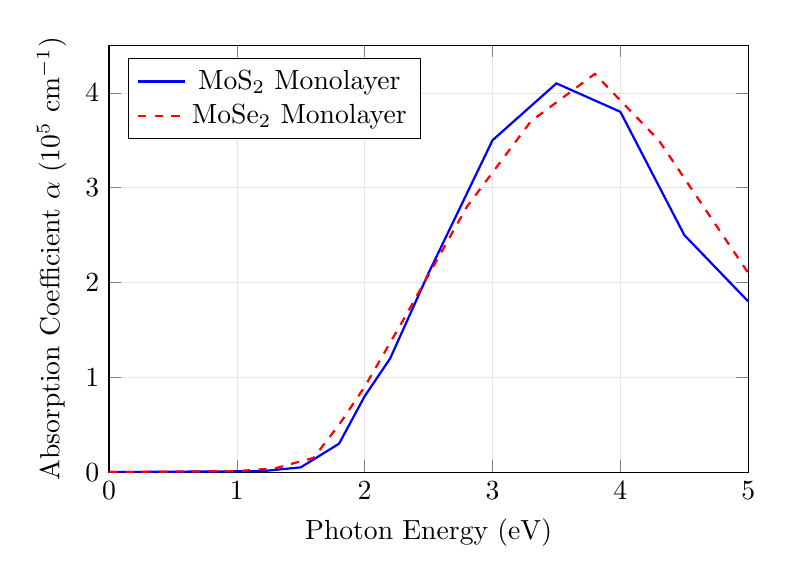
\begin{tikzpicture}
        \begin{axis}[
            width=0.8\textwidth,
            height=7cm,
            xlabel={Photon Energy (eV)},
            ylabel={Absorption Coefficient $\alpha$ ($10^5$ cm$^{-1}$)},
            xmin=0.0, xmax=5.0,
            ymin=0.0, ymax=4.5,
            legend pos=north west,
            grid=both,
            grid style={line width=.1pt, draw=gray!10},
            major grid style={line width=.2pt, draw=gray!20}
        ]
            \addplot[color=blue, thick] coordinates {
                (0.0,0.0) (1.2,0.01) (1.5,0.05) (1.8,0.3) (2.0,0.8) 
                (2.2,1.2) (2.5,2.1) (3.0,3.5) (3.5,4.1) (4.0,3.8) 
                (4.5,2.5) (5.0,1.8)
            };
            \addlegendentry{MoS$_2$ Monolayer}
            
            \addplot[color=red, dashed, thick] coordinates {
                (0.0,0.0) (1.0,0.01) (1.3,0.04) (1.6,0.15) (1.8,0.5) 
                (2.0,0.9) (2.3,1.6) (2.8,2.8) (3.3,3.7) (3.8,4.2) 
                (4.3,3.5) (5.0,2.1)
            };
            \addlegendentry{MoSe$_2$ Monolayer}
        \end{axis}
    \end{tikzpicture}
    \caption{Calculated optical absorption spectra for MoS$_2$ and MoSe$_2$ monolayers.}
    \label{fig:absorption}
\end{figure}

The absorption peaks around 3.5 eV correspond to the interband transition between the $d$-states of the transition metals and the $p$-states of the chalcogen atoms.

\section{Discussion of Physical Mechanisms}
The optical properties indicate a significant redshift of the absorption edge upon selenium substitution. This is attributed to the weaker electronegativity of Se compared to S, which raises the valence band energy levels. Our findings are in agreement with experimental measurements by \citet{novoselov2005}.
Furthermore, the enhancement of absorption in the visible range under tensile strain (discussed in Chapter~\ref{ch:results_1}) highlights the potential of these materials for flexible photovoltaic cells and solar energy harvesting.
